\documentclass[../../main.tex]{subfiles}

\begin{document}

\subsubsection{GUI}

\subfile{krop/elaboration/sags_aabning_gui_mockup}
Der vil i dette afsnit blive beskrivet hvordan sagsåbnings brugergrænsefladen er designet og implemeteret.

Gruppen valgte at alle controllerne skulle loades, fra program start af. Dette blive valgt for at skabe overskuelige, omkring hvilke controllere der er loadede, og for at gøre det nemmere at vedligeholde. For at kunne have et vilkårligt antal controller og nemt at kunne tilgå dem, bliver de opbevaret i et Map i \code{GUI}. For at kunne gemme controllerne i et Map skal de være af samme type. Derfor blev klassen \code{Controller} introduceret, denne klasse indeholder en private variable \code{stage} af typen \code{Stage}, som kan vises ved at kalde metoden \code{open()}. Sagsåbnings processen er designet så de forskellige elementer ligger i forskellige tabs. Hvert tab har sin egen controller og fxml-dokument. Og hvert tab har brug for at kende til instansen af \code{Case} som ligger i \code{GUI} klassen. For nemt at kunne give de forskellige tab-controller en reference til casen, er klassen \code{TabController} lavet. Denne klasse indeholder en private variable \code{c} af typen \code{Case} og getter- og settermetode hertil. Alle tab-controllerne arver fra \code{TabController}. Dette gør det muligt nemt at iterere igennem alle tab-controllerne og kalde \code{setCase()} på dem. På figur \ref{fig:gui_create_case} ses design diagrammet for gui'en. 

\begin{figure}[H]
  \centering
  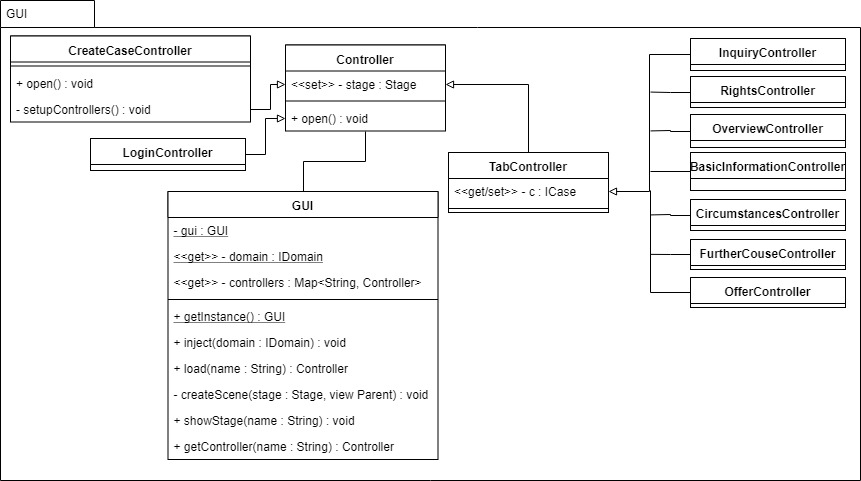
\includegraphics[scale=.15]{figurer/gui_create_case.png}
  \caption{Designdiagram over gui'en til lave en sag}
  \label{fig:gui_create_case}
\end{figure}
\end{document}
